% Options for packages loaded elsewhere
\PassOptionsToPackage{unicode}{hyperref}
\PassOptionsToPackage{hyphens}{url}
%
\documentclass[
]{article}
\usepackage{lmodern}
\usepackage{amssymb,amsmath}
\usepackage{ifxetex,ifluatex}
\ifnum 0\ifxetex 1\fi\ifluatex 1\fi=0 % if pdftex
  \usepackage[T1]{fontenc}
  \usepackage[utf8]{inputenc}
  \usepackage{textcomp} % provide euro and other symbols
\else % if luatex or xetex
  \usepackage{unicode-math}
  \defaultfontfeatures{Scale=MatchLowercase}
  \defaultfontfeatures[\rmfamily]{Ligatures=TeX,Scale=1}
\fi
% Use upquote if available, for straight quotes in verbatim environments
\IfFileExists{upquote.sty}{\usepackage{upquote}}{}
\IfFileExists{microtype.sty}{% use microtype if available
  \usepackage[]{microtype}
  \UseMicrotypeSet[protrusion]{basicmath} % disable protrusion for tt fonts
}{}
\makeatletter
\@ifundefined{KOMAClassName}{% if non-KOMA class
  \IfFileExists{parskip.sty}{%
    \usepackage{parskip}
  }{% else
    \setlength{\parindent}{0pt}
    \setlength{\parskip}{6pt plus 2pt minus 1pt}}
}{% if KOMA class
  \KOMAoptions{parskip=half}}
\makeatother
\usepackage{xcolor}
\IfFileExists{xurl.sty}{\usepackage{xurl}}{} % add URL line breaks if available
\IfFileExists{bookmark.sty}{\usepackage{bookmark}}{\usepackage{hyperref}}
\hypersetup{
  hidelinks,
  pdfcreator={LaTeX via pandoc}}
\urlstyle{same} % disable monospaced font for URLs
\usepackage{color}
\usepackage{fancyvrb}
\newcommand{\VerbBar}{|}
\newcommand{\VERB}{\Verb[commandchars=\\\{\}]}
\DefineVerbatimEnvironment{Highlighting}{Verbatim}{commandchars=\\\{\}}
% Add ',fontsize=\small' for more characters per line
\newenvironment{Shaded}{}{}
\newcommand{\AlertTok}[1]{\textcolor[rgb]{1.00,0.00,0.00}{\textbf{#1}}}
\newcommand{\AnnotationTok}[1]{\textcolor[rgb]{0.38,0.63,0.69}{\textbf{\textit{#1}}}}
\newcommand{\AttributeTok}[1]{\textcolor[rgb]{0.49,0.56,0.16}{#1}}
\newcommand{\BaseNTok}[1]{\textcolor[rgb]{0.25,0.63,0.44}{#1}}
\newcommand{\BuiltInTok}[1]{#1}
\newcommand{\CharTok}[1]{\textcolor[rgb]{0.25,0.44,0.63}{#1}}
\newcommand{\CommentTok}[1]{\textcolor[rgb]{0.38,0.63,0.69}{\textit{#1}}}
\newcommand{\CommentVarTok}[1]{\textcolor[rgb]{0.38,0.63,0.69}{\textbf{\textit{#1}}}}
\newcommand{\ConstantTok}[1]{\textcolor[rgb]{0.53,0.00,0.00}{#1}}
\newcommand{\ControlFlowTok}[1]{\textcolor[rgb]{0.00,0.44,0.13}{\textbf{#1}}}
\newcommand{\DataTypeTok}[1]{\textcolor[rgb]{0.56,0.13,0.00}{#1}}
\newcommand{\DecValTok}[1]{\textcolor[rgb]{0.25,0.63,0.44}{#1}}
\newcommand{\DocumentationTok}[1]{\textcolor[rgb]{0.73,0.13,0.13}{\textit{#1}}}
\newcommand{\ErrorTok}[1]{\textcolor[rgb]{1.00,0.00,0.00}{\textbf{#1}}}
\newcommand{\ExtensionTok}[1]{#1}
\newcommand{\FloatTok}[1]{\textcolor[rgb]{0.25,0.63,0.44}{#1}}
\newcommand{\FunctionTok}[1]{\textcolor[rgb]{0.02,0.16,0.49}{#1}}
\newcommand{\ImportTok}[1]{#1}
\newcommand{\InformationTok}[1]{\textcolor[rgb]{0.38,0.63,0.69}{\textbf{\textit{#1}}}}
\newcommand{\KeywordTok}[1]{\textcolor[rgb]{0.00,0.44,0.13}{\textbf{#1}}}
\newcommand{\NormalTok}[1]{#1}
\newcommand{\OperatorTok}[1]{\textcolor[rgb]{0.40,0.40,0.40}{#1}}
\newcommand{\OtherTok}[1]{\textcolor[rgb]{0.00,0.44,0.13}{#1}}
\newcommand{\PreprocessorTok}[1]{\textcolor[rgb]{0.74,0.48,0.00}{#1}}
\newcommand{\RegionMarkerTok}[1]{#1}
\newcommand{\SpecialCharTok}[1]{\textcolor[rgb]{0.25,0.44,0.63}{#1}}
\newcommand{\SpecialStringTok}[1]{\textcolor[rgb]{0.73,0.40,0.53}{#1}}
\newcommand{\StringTok}[1]{\textcolor[rgb]{0.25,0.44,0.63}{#1}}
\newcommand{\VariableTok}[1]{\textcolor[rgb]{0.10,0.09,0.49}{#1}}
\newcommand{\VerbatimStringTok}[1]{\textcolor[rgb]{0.25,0.44,0.63}{#1}}
\newcommand{\WarningTok}[1]{\textcolor[rgb]{0.38,0.63,0.69}{\textbf{\textit{#1}}}}
\usepackage{graphicx,grffile}
\makeatletter
\def\maxwidth{\ifdim\Gin@nat@width>\linewidth\linewidth\else\Gin@nat@width\fi}
\def\maxheight{\ifdim\Gin@nat@height>\textheight\textheight\else\Gin@nat@height\fi}
\makeatother
% Scale images if necessary, so that they will not overflow the page
% margins by default, and it is still possible to overwrite the defaults
% using explicit options in \includegraphics[width, height, ...]{}
\setkeys{Gin}{width=\maxwidth,height=\maxheight,keepaspectratio}
% Set default figure placement to htbp
\makeatletter
\def\fps@figure{htbp}
\makeatother
\setlength{\emergencystretch}{3em} % prevent overfull lines
\providecommand{\tightlist}{%
  \setlength{\itemsep}{0pt}\setlength{\parskip}{0pt}}
\setcounter{secnumdepth}{-\maxdimen} % remove section numbering

\date{}

\begin{document}

\hypertarget{header-n0}{%
\section{Oct 22 Tue}\label{header-n0}}

\hypertarget{header-n2}{%
\subsection{SE-302::Compilers}\label{header-n2}}

继续说 Activation Records。

上节课说的,我们通过一个叫做 "static link" 的东西来实现跨 Scope
访问。跨多少层静态嵌套层,就需要多少次寻址。

这个 static link 需要被传递。如何?我们默认它是每个函数的第一个参数。

\hypertarget{header-n6}{%
\subsubsection{static link}\label{header-n6}}

实际上只是一个访问「上一层函数」的 Frame(栈底)的指针。

但实际上我们怎么使用?

\hypertarget{header-n9}{%
\paragraph{Usage}\label{header-n9}}

在发现一个当前 Scope 里找不到的符号的时候,我们就从 static link
着手往上一层的 Frame
寻找,找我们需要的那个符号;如果这一层还是没有,就继续通过它的「首位隐形参数」寻找继上层的
Frame。

所有上面这些操作都是需要在编译期生成实际指令的。

\hypertarget{header-n12}{%
\paragraph{P.S.}\label{header-n12}}

一个会被自己的孩子 Scope 访问的局部变量是必须进栈的。

\hypertarget{header-n14}{%
\subsubsection{display}\label{header-n14}}

static link 访存次数太多了。有没有好点的办法?

display 学名是嵌套层次显示表。本质上就是一个全局数组
\texttt{array}。\texttt{array{[}i{]}}
是一根指针,指向的是最近一次进入的静态嵌套深度为 \texttt{i} 的栈位置。

\hypertarget{header-n17}{%
\paragraph{Mutable}\label{header-n17}}

display 是一个动态改变的表。随着调用过程的深入浅出,display 会随时改变。

\hypertarget{header-n19}{%
\paragraph{Quick}\label{header-n19}}

在我们已经知道嵌套层次深度的时候,不再需要像是 static link
一样的多次奔波。只需要做一次数组的访问就可以,无论嵌套层次深度差有多少。

\hypertarget{header-n21}{%
\subsubsection{λ Lifting}\label{header-n21}}

Lambda Lifting。这是个什么主意呢?

\hypertarget{header-n23}{%
\paragraph{Idea}\label{header-n23}}

对于 \texttt{g} 调用一个函数 \texttt{f} 时,把函数
\texttt{f}(及其内部嵌套的函数)使用到的 \texttt{g}
中的变量都作为额外的参数传给 \texttt{f} 。

反正要用到哪些外部变量,我们都(在编译期)知道了。

\hypertarget{header-n26}{%
\subsubsection{What about a Tiger?}\label{header-n26}}

本书采用了 static link 的实现方法。

\hypertarget{header-n28}{%
\subsubsection{Frame}\label{header-n28}}

栈帧:Tiger 是怎么实现的?

\hypertarget{header-n30}{%
\paragraph{Incompatible}\label{header-n30}}

比较大的问题是:不同的环境存在不同的栈帧布局。这也很正常:64 位跟 32
位生成代码的栈帧肯定具有不同的布局:指针长度都不同。

为了实现编译器的可移植性,我们最好不要直接写 Machine Dependent
的代码到编译器中,否则要支持一个新的平台,代价会太大。

\hypertarget{header-n33}{%
\paragraph{Abstract Methods}\label{header-n33}}

解决方法就是:使用抽象方法来实现栈帧,隐藏底部具体(机器相关)实现。

这样对每一种 arch,只需要实现一遍 Abstract Method
就能完成移植了,而不需要改动 Compilers 的逻辑部分。

\hypertarget{header-n36}{%
\paragraph{Frame Structure}\label{header-n36}}

Abstract Methods 在 \texttt{\textless{}frame.h\textgreater{}} 中被定义。

\begin{Shaded}
\begin{Highlighting}[]
\CommentTok{/* frame.h */}
\KeywordTok{typedef} \KeywordTok{struct}\NormalTok{ F_frame_ *F_frame ;}
\NormalTok{F_frame F_newFrame(Temp_label name, U_boolList formals);}
\end{Highlighting}
\end{Shaded}

一个关键信息是 Formal Parameters(形式参数)和在栈上分配的临时变量。

\hypertarget{header-n40}{%
\paragraph{Escape}\label{header-n40}}

那么 \texttt{U\_boolList} 是个啥?这是一串儿 Bool 标记,对应到每个形参;

它指定的是 Escape 与否。

如果 Escape 为真,则此参数不可被放入寄存器,而必须被放在栈上。

因为他要被用于后续的 escaping static link。

否则如果 Escape 为假,则无需在意其是否被放入寄存器或是栈上。

\hypertarget{header-n46}{%
\paragraph{Syntax}\label{header-n46}}

留意一下:U\_boolList 跟 Lab 3 里那堆东西一样;不是一个好好的
List,而是个链表,写起来看起来都难受\ldots\ldots{}

要声明一个三形参的函数
\texttt{g(arg1,\ arg2,\ arg3)},标记她们除了第一个逃逸外其他的都不逃逸,我们得这么开
Frame:

\begin{Shaded}
\begin{Highlighting}[]
\NormalTok{F_newFrame(g, }
\NormalTok{	U_BoolList(TRUE,}
\NormalTok{		U_BoolList(FALSE,}
\NormalTok{			U_BoolList(FALSE, NULL)}
\NormalTok{		)}
\NormalTok{	)}
\NormalTok{);}
\end{Highlighting}
\end{Shaded}

\hypertarget{header-n50}{%
\subparagraph{\texorpdfstring{Swift
\texttt{@escaping}}{Swift @escaping}}\label{header-n50}}

\begin{verbatim}
func foo(strList: @escaping String[]) {
    
}
\end{verbatim}

Swift 的 \texttt{@escaping} Annotation 就表达了这个意思。

\hypertarget{header-n53}{%
\paragraph{Variables}\label{header-n53}}

同样对于一个临时变量来说,我们也存在「是放在栈上?」或「放在寄存器里?」这样的不确定。

因此为了记录这种不同并将其统一,我们设计了这种数据结构:

\begin{Shaded}
\begin{Highlighting}[]
\CommentTok{/* mipsframe.h */}
\PreprocessorTok{#include “frame.h”}
\KeywordTok{struct}\NormalTok{ F_access_ \{}
	\KeywordTok{enum}\NormalTok{ \{inFrame, inReg\} kind;}
	\KeywordTok{union}\NormalTok{ \{}
		\DataTypeTok{int}\NormalTok{ offset;			}\CommentTok{/* InFrame */}
\NormalTok{		Temp_temp reg;		}\CommentTok{/* InReg */}
\NormalTok{	\} u;}
\NormalTok{\};}
\KeywordTok{struct}\NormalTok{ Temp_temp_ \{}\DataTypeTok{int}\NormalTok{ num;\};}
\AttributeTok{static}\NormalTok{ F_access Inframe(}\DataTypeTok{int}\NormalTok{ offset);}
\AttributeTok{static}\NormalTok{ F_access InReg(Temp_temp reg);}
\end{Highlighting}
\end{Shaded}

\hypertarget{header-n57}{%
\subparagraph{\texorpdfstring{\texttt{F\_access\_}
kind}{F\_access\_ kind}}\label{header-n57}}

留意到 inFrame 状态和 inReg 状态需要不同的位置记录法,我们使用了经典的
kind + union 记录法。

offset 对应的是 kind = inFrame,记录着这个变量和栈底的距离;

为什么是栈底?因为栈是倒长的,call 的时候栈底就定了。

reg 对应的是 kind = inReg,对应一枚虚拟寄存器。

\hypertarget{header-n62}{%
\subparagraph{\texorpdfstring{\texttt{F\_allocLocal}}{F\_allocLocal}}\label{header-n62}}

调用 \texttt{F\_allocLocal} 来分配临时/局部变量。

\begin{Shaded}
\begin{Highlighting}[]
\NormalTok{F_allocLocal(foo, TRUE);}
\CommentTok{/* 来把 foo 分配在栈上。 */}

\NormalTok{F_allocLocal(baz, FALSE);}
\CommentTok{/* 尽量把 baz 分配在寄存器里。 */}
\end{Highlighting}
\end{Shaded}

\hypertarget{header-n65}{%
\subparagraph{\texorpdfstring{Temp\emph{temp}
}{Temptemp }}\label{header-n65}}

就是上面的虚拟寄存 器:相比于实际的寄存器而言,它有无限多个。

\hypertarget{header-n67}{%
\paragraph{Formals}\label{header-n67}}

\begin{Shaded}
\begin{Highlighting}[]
\CommentTok{/* frame.h */}
\KeywordTok{typedef} \KeywordTok{struct}\NormalTok{ F_access *F_access ;}
\KeywordTok{typedef}  \KeywordTok{struct}\NormalTok{ F_accessList_ *F_accessList;}
\KeywordTok{struct}\NormalTok{ F_accessList_ \{ F_access head; F_accessList tail; \};}
\NormalTok{F_accessList F_formals(F_frame f);}
\end{Highlighting}
\end{Shaded}

留意到:F\_formals 拿到的一串 k 都是从
Callee,也就是从被调用者的角度、内部来看的。

F\_formals() extracts a list of k ``accesses'' denoting the locations
w6here the formal parameters will be kept at run time as seen from
inside the callee

\hypertarget{header-n71}{%
\paragraph{Caller \& Callee}\label{header-n71}}

主要的问题就是 Caller 跟 Callee 所看到的形参列表怎么统一。在 Caller call
Callee
的时候,我们需要把视角进行转换,从调用者的视角转变成被调用者的视角,并开始向下执行。

\hypertarget{header-n73}{%
\subparagraph{x86\_32}\label{header-n73}}

好办;所有参数全部进栈。而且 x86\_32
有两根指针用来管理栈:栈顶指针和栈底指针。

\hypertarget{header-n75}{%
\subparagraph{Sparc}\label{header-n75}}

类似于 MIPS。

\hypertarget{header-n77}{%
\subparagraph{MIPS}\label{header-n77}}

\hypertarget{header-n78}{%
\paragraph{Nested Block}\label{header-n78}}

有一些语言(Tiger 也有)Nested Block 的说法:被 Braces
包围的语句块可以包含 Nested Variables Declaration。

但是我们并不会为了这一个 Brace Block 去额外开一个
Frame;它还是被开在跟上级一样的 Frame 里的。

也就是说在我们离开这个 Brace Block 的时候,

这个局局部变量会被忘记「forgotten」,但不会消失「disappear」。

他会继续隐形地活到 Frame 的上下文中止。

\hypertarget{header-n84}{%
\subsection{SE-227::CSE}\label{header-n84}}

今天我们目前仍然处于 IP Layer。

NetGate/GateWay: 内网发送网络请求时,如何让外网 Server 找到请求者的 IP?

Answer: 内外网转换时,也就是在 Gateway 处,维护了一个 Network Address
Translation(NAT)表。

\hypertarget{header-n88}{%
\subsubsection{Case Study::Ethernet Mapping}\label{header-n88}}

Ethernet 是啥?本身是想要取代 Internet 的。可惜没成。现在只能用来做本地
Link Layer 的一部分。

我们来分析分析这个案例吧。

\hypertarget{header-n91}{%
\paragraph{Mapping?}\label{header-n91}}

Key ⥋ Value 的对应映射。

IP 地址大家都熟悉:IPv4 的 23.45.56.67,只有 32 位;IPv6 更长些。

而 Ethernet 地址呢,长相类似于 MAC 地址的
12:34:56:78:90:ab。比较起来,它有 48 位。

\hypertarget{header-n95}{%
\paragraph{CSMA/CD?}\label{header-n95}}

Ethernet 具有这样的性质:

Carrier Sense Multiple Access with Collision
Detection。带有冲突检测的载波聚合访问。

留意到 Ethernet 不需要进行 Forwarding;

在我发现这个包不是给我的时候,不需要做任何特殊事情;

因为这个包是广播的;我收到了别人肯定也收到了。

如果这个包是给我的,拿来就好了。

跟 Internet 不太一样;

在 Internet
你拿出一个包发现不是给自己的,还需要再把它给转发出去给接下来的人。否则这包就丢了。

也因为这种性质,我们可以监听所有包。

\hypertarget{header-n105}{%
\paragraph{Half/Full Duplex?}\label{header-n105}}

全双工:可以同时收发包;没有包大小限制。

半双工:有包大小限制(为了做冲突检测,防止包太小还没检查出来就发了);发生冲突时需要重发。

\hypertarget{header-n108}{%
\paragraph{Checksum?}\label{header-n108}}

每个 Package 都包含 32 位的 Checksum 校验和位。

\hypertarget{header-n110}{%
\paragraph{Ethernet Address?}\label{header-n110}}

注意在 Router 之间发送的时候,包头里的 Ethernet Address 是一直在变化的。

如果要跨 Ethernet
组发包,就必须以我组路由器的身份,发给隔壁组的路由器;然后再由隔壁组的路由器构造新的
Ethernet 请求,这样就实现了跨网传送。

\hypertarget{header-n113}{%
\paragraph{ARP?}\label{header-n113}}

Address Resolution Protocol。

在这个 Ethernet
网络里出现一个大家都不认识的网络节点;路由器就会开一个广播:谁认识这位?

所有人都去查一下记录本;如果不认识就不发包;认识就把它广播出来。大家就都记下来了。

\hypertarget{header-n117}{%
\paragraph{RARP?}\label{header-n117}}

Reversed ARP。

\hypertarget{header-n119}{%
\subsubsection{ARP Spoofing}\label{header-n119}}

ARP 欺骗攻击:如何进行?

\hypertarget{header-n121}{%
\paragraph{Procedure}\label{header-n121}}

ARP欺骗的运作原理是由攻击者发送假的 ARP
数据包到网络上,尤其是送到网关上。其目的是要让送至特定的IP地址的流量被错误送到攻击者所取代的地方。因此攻击者可将这些流量另行转送到真正的网关(被动式数据包嗅探,passive
sniffing)或是篡改后再转送(中间人攻击,man-in-the-middle
attack)。攻击者亦可将ARP数据包导到不存在的 MAC
地址以达到拒绝服务攻击的效果,例如 netcut 软件。

例如某一的IP地址是\texttt{192.168.0.254},其MAC地址为\texttt{00-11-22-33-44-55},网络上的电脑内ARP表会有这一笔ARP记录。攻击者发动攻击时,会大量发出已将\texttt{192.168.0.254}的MAC地址篡改为\texttt{00-55-44-33-22-11}的ARP数据包。那么网络上的电脑若将此伪造的ARP写入自身的ARP表后,电脑若要透过网络网关连到其他电脑时,数据包将被导到\texttt{00-55-44-33-22-11}这个MAC地址,因此攻击者可从此MAC地址截收到数据包,可篡改后再送回真正的网关,或是什么也不做,让网络无法连线。

\href{https://zh.wikipedia.org/wiki/File:Ethernet_Type_II_Frame_format.svg}{\includegraphics{https:////upload.wikimedia.org/wikipedia/commons/thumb/1/13/Ethernet_Type_II_Frame_format.svg/500px-Ethernet_Type_II_Frame_format.svg.png}}

Ethernet数据包,ARP欺骗会篡改数据包标头中的Source
MAC地址(绿色段)以欺骗网络上的电脑及设备

\textbf{简单案例分析}:这里用一个最简单的案例来说明ARP欺骗的核心步骤。假设在一个LAN里,只有三台主机A、B、C,且C是攻击者。

\begin{enumerate}
\def\labelenumi{\arabic{enumi}.}
\item
  攻击者聆听局域网上的MAC地址。它只要收到两台主机洪泛的ARP
  Request,就可以进行欺骗活动。
\item
  主机A、B都洪泛了ARP
  Request.攻击者现在有了两台主机的IP、MAC地址,开始攻击。
\item
  攻击者发送一个ARP Reply给主机B,把此包protocol header里的sender
  IP设为A的IP地址,sender mac设为攻击者自己的MAC地址。
\item
  主机B收到ARP Reply后,更新它的ARP表,把主机A的MAC地址(IP\emph{A,
  MAC}A)改为(IP\emph{A, MAC}C)。
\item
  当主机B要发送数据包给主机A时,它根据ARP表来封装数据包的Link报头,把目的MAC地址设为MAC\emph{C,而非MAC}A。
\item
  当交换机收到B发送给A的数据包时,根据此包的目的MAC地址(MAC\_C)而把数据包转发给攻击者C。
\item
  攻击者收到数据包后,可以把它存起来后再发送给A,达到偷听效果。攻击者也可以篡改数据后才发送数据包给A,造成伤害。
\end{enumerate}

\hypertarget{header-n142}{%
\paragraph{Defense}\label{header-n142}}

\begin{itemize}
\item
  放弃 ARP 协议广播,写死这张表

  \begin{itemize}
  \item
    死板
  \item
    难搞
  \item
    慢
  \end{itemize}
\item
  Arpwatch

  \begin{itemize}
  \item
    观察识别这种 ARP spoofing 的异常流量
  \item
    Ban IP
  \item
    请喝茶
  \end{itemize}
\end{itemize}

\hypertarget{header-n162}{%
\subsubsection{Routing}\label{header-n162}}

Routing Table 目前已经不可能被存储在一个中心了。因为网络已经太大了。

总归只能用一些碎片的网络来实现我们的请求。

每一个 Router
要么知道这个包该去哪,要么知道在不知道这个包该去哪的时候该把它往哪里送。

而且,我们还需要尽量保证 minimum-cost 的道路,否则花费太大也不好。

\hypertarget{header-n167}{%
\paragraph{Switcher}\label{header-n167}}

交换机,本质上也就是特别一点的计算机。

分布式的 Routing: 3 Steps in General

\begin{enumerate}
\def\labelenumi{\arabic{enumi}.}
\item
  先给邻居说一句 HELLO!通过大家都接受的 HELLO protocol。
\item
  这些节点又去了解自己可达的节点,通过 ADVERTISEMENTS。
\item
  通过图论的一些知识来决定 Minimum-Cost 的发包路线。
\end{enumerate}

\hypertarget{header-n177}{%
\paragraph{Types}\label{header-n177}}

主要有两类 Routing 的 Protocol:

\hypertarget{header-n179}{%
\subparagraph{Protocol 1 - Link-state}\label{header-n179}}

每一个节点都去告诉所有人:

我认识 foo,我跟他的距离是 1\ldots{}

我认识 bar,我跟他的距离是 5\ldots{}

在大家广告完毕之后,每个人都有了一个自己心里的拓扑图。

\begin{quote}
这必要吗?
\end{quote}

这样就可以用 Dijkstra 等等算法来决定发包路线了。

只是 Telling Everyone 这件事消耗网络资源实在有点大\ldots{}

在网络不太复杂的情况下,LINK-STATE 还是可以用的。

基本一所学校还是够用的;上升到一个市基本就不成了。

\hypertarget{header-n190}{%
\subparagraph{Protocol 2 - Distance-Vector}\label{header-n190}}

「传八卦」「要悄悄说」

每个节点只告诉自己的\textbf{邻居们}自己到所有已知距离的结点的距离。

直到最后,到达一个状态,每个节点知道的事情是:

\begin{enumerate}
\def\labelenumi{\arabic{enumi}.}
\item
  自己到自己所有邻居的距离;
\item
  自己的邻居到所有已知节点的距离(但并不知道是直连还是绕路,也不知道个中拓扑信息)。
\end{enumerate}

不要大张旗鼓告诉所有人了;省点流量吧。

事实上,对于单个节点知道整块拓扑图,意义是不大的。

我们只要大概地知道对于每个终点的包,往哪一边發更快就够了。

要发也是我往邻居那边发,接下来的事给邻居考虑就好了。

\hypertarget{header-n203}{%
\paragraph{Infinity}\label{header-n203}}

当 A 与 B 之间没有通路的时候,该怎么告诉?

一般会说 A =\textgreater{} B 的代价是 INFINITY。

但考虑这么一个问题:

在一条通路中断的时候(曾经不是 INFINITY,后来因为种种原因中断了),

该如何通知其他节点「我的通路断掉了,不要再把包发给我了」?

因为如果不去声明这一点,就可能会产生死循环。

\begin{figure}
\centering
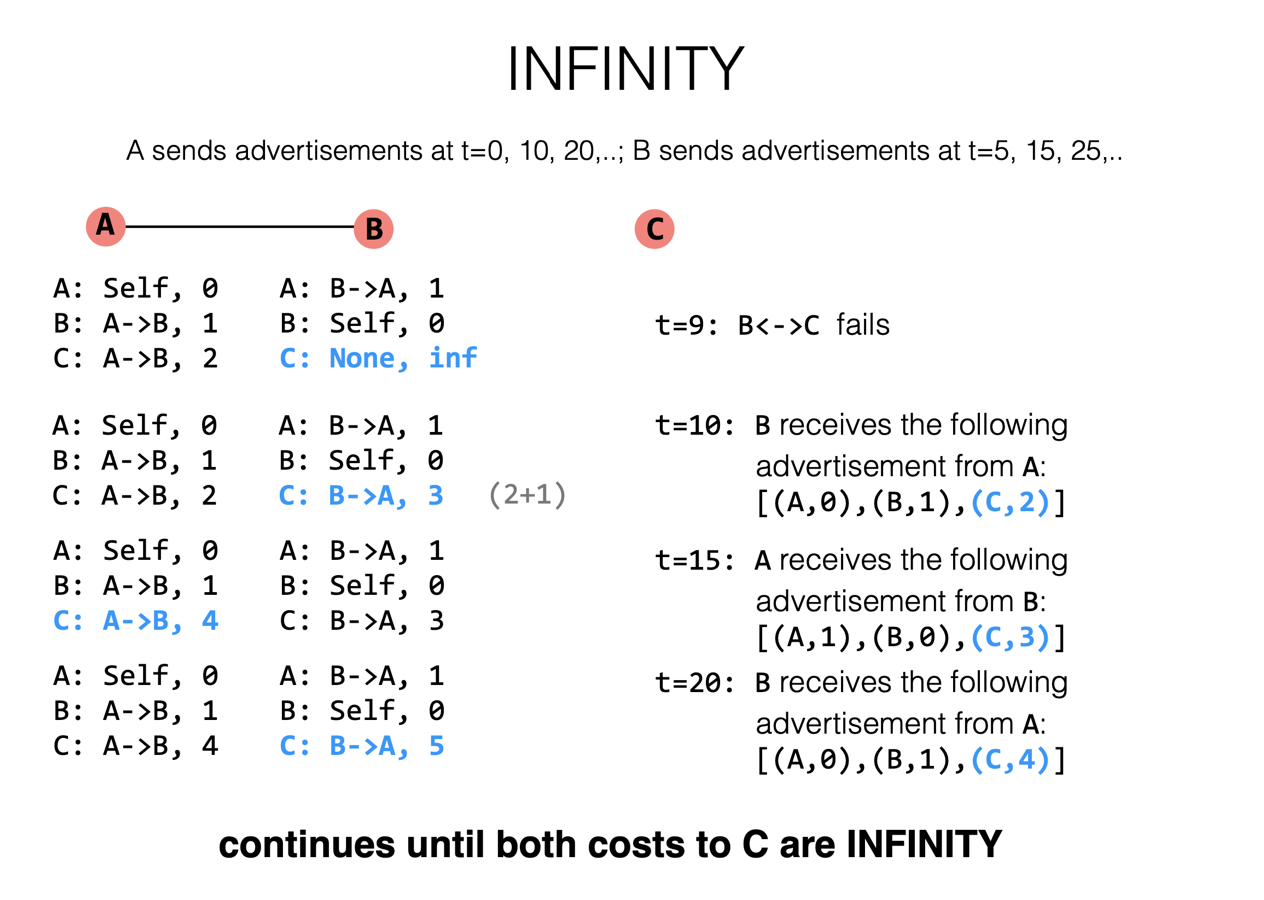
\includegraphics{https://github.com/yuetsin/2019-2020-autumn-semester/blob/master/10-october/22.assets/image-20191022112329871.png?raw=true}
\caption{}
\end{figure}

\hypertarget{header-n211}{%
\paragraph{Rule}\label{header-n211}}

不要声明一个通路指向他的来源。

否则会产生死循环。

Split Horizon:不要把发给我的包再发回给你。否则待会还得来我这里。

然而这个规则并不是那么容易实现:Failure 和 Infinite
Loop(非直接的循环圈)也很难 Handle。

主要原因就是 Distance-Vector
携带的信息太少了,完全不包括任何拓扑结构的信息。

Internet 这么大的规模,该怎么解决上面的这些问题呢?

• \textbf{Path-vector Routing}

-- Advertisements include the path, to better detect routing loops

• \textbf{Hierarchy of Routing}

-- Route between \textbf{regions}, and then within a region

Hierarchy 解决规模化的问题还是重要的。

• \textbf{Topological Addressing}

-- Assign addresses in contiguous blocks to make advertisements smaller

\end{document}
